\chapter{Hardware und Software}
Dieses Kapitel führt die gegebenen und verwendeten Hard- und Software Komponenten in dieser Arbeit auf.

\section{Der Kaffeevollautomat}
Der "`Jura Impressa S9"', siehe Abbildung \ref{fig:Kaffeevollautomat}, ist ein Kaffeevollautomat mit fünf Kaffeebezugstasten: Spezialkaffee, 1 große Tasse Kaffee, 2 große Tassen Kaffee, 1 kleine Tasse Kaffee und 2 kleinen Tassen Kaffee.
Auf der rechten Seite befinden sich Bedienelemente für heißes (Tee-)Wasser und Wasserdampf zum Milch Aufschäumen.

\begin{figure}
  \begin{center}
    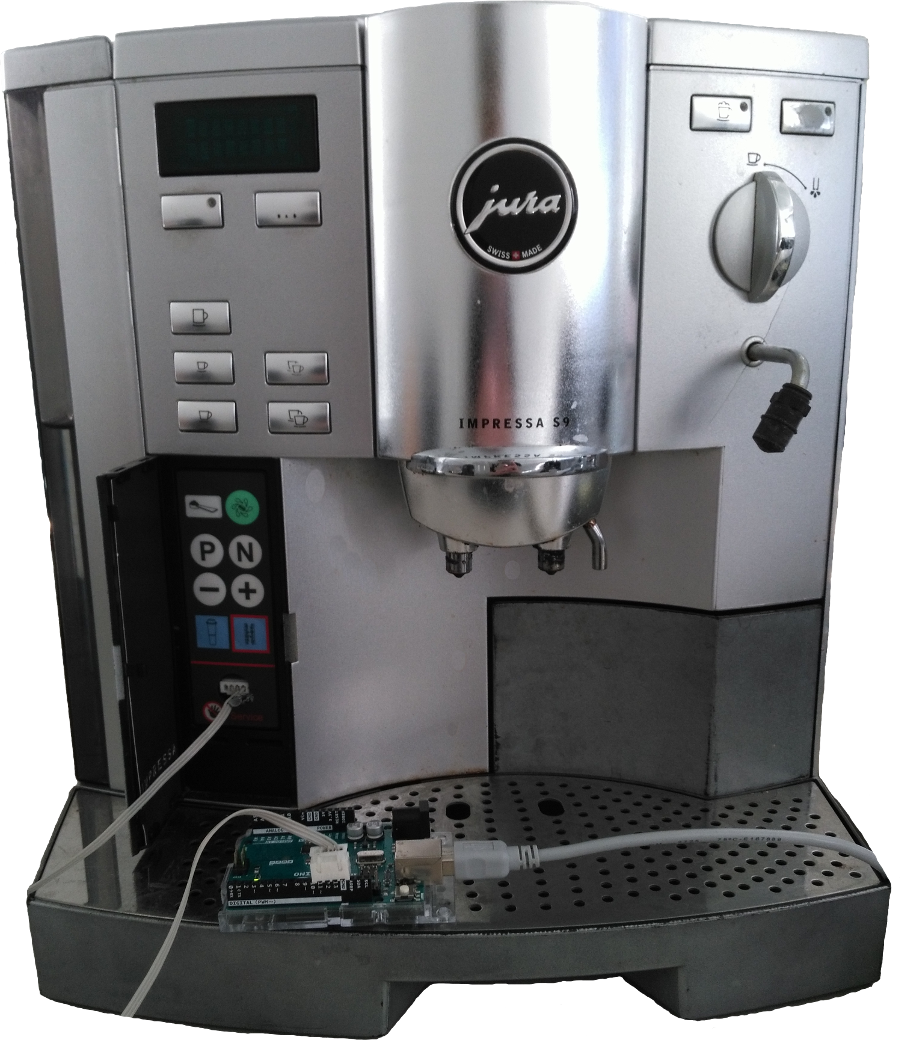
\includegraphics[scale=0.2]{images/Jura-Impressa-S9-small}
    \caption{Jura Impressa S9 -- Kaffeevollautomat}
    \label{fig:Kaffeevollautomat}
  \end{center}
\end{figure}

\subsection{Aufbau und Verkabelung}
Interessanter wird es hinter der linken Wartungsklappe an der Vorderseite des Kaffeevollautomaten.
Dort befindet sich neben mehreren Menü-Tasten auch eine serielle Schnittstelle.
Über ein eigenes \ac{UART} Protokoll, siehe Kapitel \ref{subsec:SerielleKommunikation}, kann hierüber mit der Maschine kommuniziert werden.

Abbildung \ref{fig:KaffeevollautomatPins} illustriert die Pinbelegung.
Die 5 Volt Leitung käme für ein autark laufendes Projekt in Betracht.
In dieser Arbeit bezieht der Arduino seine Versorgungsspannung über den am USB Kabel befindlichen Computer.
Der Kaffeevollautomat wird dirkt mit der Netzspannung versorgt.
Von \texttt{TX} nach \texttt{RxD} werden Befehle an den Kaffeevollautomaten verschickt.
Auf der Rückrichtung von \texttt{TxD} nach \texttt{RX} werden Antworten des Kaffeevollautomaten gelesen.
\texttt{GND} ist abschließend die gemeinsame Erdung und Bezugsleitung für die serielle Kommunikation.
Auf der Abbildung kreuzen sich die Leitungen \texttt{RxD} und \texttt{GND} am Stecker auf Seiten des Kaffeevollautomaten.
\texttt{GND} ist über eine schwarze Markierung gekennzeichnet.

Ein Arduino Uno übersetzt als "`Man in the middle"' die bekannten Kommandos in das Format der Kaffeemaschine.
Sie serielle Kommunikation läuft über die Pins Nummer 12 und 13.
Über eine weitere serielle Verbindung per USB lässt sich der Arduino ansteuern.

Aus Sicht des Computers ist der Arduino ein Gerätelaufwerk unter \texttt{/dev/ttyACM0} mit einer Baudrate von 9600.
Diese Zahl findet sich zu Beginn des Arduino Skrips (Fußnote \ref{GitlabProject_CoffeeMachine}) wieder.

\begin{figure}
  \begin{center}
    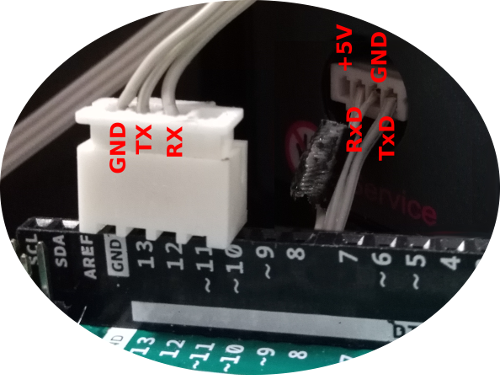
\includegraphics[scale=0.3]{images/Jura-Arduino-Pins-beschriftet-small}
    \caption{Pinbelegung: Jura Impressa S9 -- Arduino Uno}
    \label{fig:KaffeevollautomatPins}
  \end{center}
\end{figure}

\subsection{Kommandos}
Die Tabelle~\ref{tbl:kommandos} zeigt die Befehlsgruppen, sowie ausgewählte Befehle, die der Kaffeevollautomat versteht.
Einige Befehle, die aus weiteren Projekten mit Maschinen der S-Reihe bekannt sind, sind in dieser "`Jura Impressa S9"' leider nicht implementiert.

\begin{tuhhtable}
  \footnotesize\centering
  \begin{tabular}[tp]{L{.22\textwidth}L{.48\textwidth}L{.18\textwidth}}
%
  \THc{1}{c}{Kommando} & \THc{1}{c}{Beschreibung} & \THc{1}{c}{Rückgabewert} \\
%
  \TRx{3}{l}{Betriebszustand (AN:<id>)}\\
  \abovebodyrule
  AN:01    & Einschalten        & ok:    \\\TRc
  AN:02    & Ausschalten        & ok:    \\
  AN:03    & Display Test       & ok:    \\\TRc
  AN:<id>  & u.v.m.             & ok:    \\
  \belowbodyrule
%
  \TRx{3}{l}{Bezugstaste (FA:<id>)}\\
  \abovebodyrule
  FA:02    & Gerät spülen       & ok:    \\\TRc
  FA:0C    & Spezialkaffee      & ok:    \\
  FA:<id>  & u.v.m.             & ok:    \\\TRc
  \belowbodyrule
%
  \TRx{3}{l}{Steuerungskomponenten (FN:<id>)}\\
  \abovebodyrule
  FN:<id>  & Pumpen, Heizung, u.v.m & ok:    \\\TRc
  \belowbodyrule
%
  \TRx{3}{l}{Eingabestatus*}\\
  \abovebodyrule
  IC:      & Eingaben auslesen* &        \\\TRc
  \belowbodyrule
%
  \TRx{3}{l}{Spiele Musik (easter egg)*}\\
  \abovebodyrule
  PM:      & Play music*        &        \\\TRc
  \belowbodyrule
%
  \TRx{3}{l}{Speicherzugriff}\\
  \abovebodyrule
  RE:<address> & Liest 2 Byte EEPROM Speicher   & re:[0000-FFFF] \\\TRc
  WE:<address>,<value> & Schreibt 2 Byte in EEPROM & ok:         \\
  RT:<address> & Liest eine Zeile EEPROM        & rt:[0-F 64x]   \\\TRc
  RR:<address> & Liest eine Zeile RAM           & rr:[0-F 32x]   \\
  \belowbodyrule
%
  \TRx{3}{l}{Sperrung}\\
  \abovebodyrule
  ?M3      & Aktiviert den Inkassomodus         & ?ok            \\\TRc
  ?M1      & Deaktiviert den Inkassomodus       & ?ok            \\
  \belowbodyrule
%
  \TRx{3}{l}{Display}\\
  \abovebodyrule
  ?D0      & Standard Displaytext zurück setzen & ?ok            \\\TRc
  ?D1[A-Z 8-11x] & Displaytext Zeile 1          & ?ok            \\
  ?D2[A-Z 8-11x] & Displaytext Zeile 2          & ?ok            \\\TRc
  \belowbodyrule
%
  \TRx{3}{l}{Aktion an der Kaffeemaschine}\\
  \abovebodyrule
           & 1 kleiner Kaffee (Produkt 1)       & ?PAE         \\\TRc
           & 2 kleine Kaffees (Produkt 2)       & ?PAF         \\
           & 1 großer Kaffee  (Produkt 3)       & ?PAA         \\\TRc
           & 2 große Kaffees  (Produkt 4)       & ?PAB         \\
           & Spezialkaffe     (Produkt 7)       & ?PAG         \\\TRc
           & Dampf            (Produkt 6)       & ?PAI         \\
           & 1 Dampfportion   (Produkt 5)       & ?PAJ         \\\TRc
           & 1 Tasse Tee      (Produkt 8)       & ?PAK         \\
  \belowbodyrule
%
  \TRx{3}{l}{* leider nicht alles in der Jura Impressa S9 implementiert, siehe weitere Geräte der S-Reihe}\\
%
  \end{tabular}
  \caption{Befehlsübersicht der Jura Kaffeevollautomaten (S-Reihe)}
  \label{tbl:kommandos}
\end{tuhhtable}


\section{Bibliotheken}
Bibliotheken, hiermit sind "`libraries"' und "`frameworks"' gemeint, bieten eine Sammlung von Unterprogrammen und Routinen für eine begrenzte Aufgabe.
In der aktuellen Version bieten sie nicht nur leicht zugänglichle Aufrufe, sondern sind auch sicher und robust.

\subsection{Serielle Kommunikation}\label{subsec:SerielleKommunikation}
Aus dem Projekt "`CoffeeMachine"'\footnote{\label{GitlabProject_CoffeeMachine}\url{https://collaborating.tuhh.de/e-17/General/CoffeeMachine}} stammt das Programm des Arduino UNO zum Kodieren der \ac{UART} Kommandos.
Die an den Kaffeevollautomaten adressierten Bytes (ASCII-Zeichen für Zeichen der Befehle aus der Kommando Tabelle~\ref{tbl:kommandos}), bestehend aus seinen acht Bits, werden in je vier Bytes aufgeteilt.
Die dritte und sechste Stelle der neuen Bytes repräsentieren je zwei Bits des ursprünglichen Bytes.
Bei der Übertragung an den Kaffeevollautomaten werden die restlichen Bits mit Nullen aufgefüllt.
Abbildung \ref{fig:uart} veranschaulicht dies an dem ersten Byte des Einschaltbefehls, die entsprechende ASCII-Kodierung ist in Abbildung \ref{tbl:Displaysymbole} der zweiten und dritten Spalte zu entnehmen.
Die Kodierung der, von dem Kaffeevollautomaten kommenden, Bytes erfolgt analog.
Laut "`Protocoljura"'\footnote{\url{http://protocoljura.wiki-site.com/index.php/Protocol_to_coffeemaker}} bestehen die irrelevanten Bits der ankommenden Bytes aus einer Null und weiteren fünf Einsen pro Byte.

Vier Bytes kodieren ein ASCII Zeichen und werden fortan als Gruppe bezeichnet.
Zwischen jeder Gruppe gibt es eine Verzögerung von 8ms.
Diese Verzögerung begrenzt hauptsächlich die Übertragungsgeschwindigkeit, was in Abschnitt \ref{subsec:zugangSeriellDirekt} diskutiert wird.

Die jetzt vorhandene Umgebung kann bereits über den seriellen Monitor der Arduino IDE genutzt werden.

\begin{figure}
  \begin{center}
    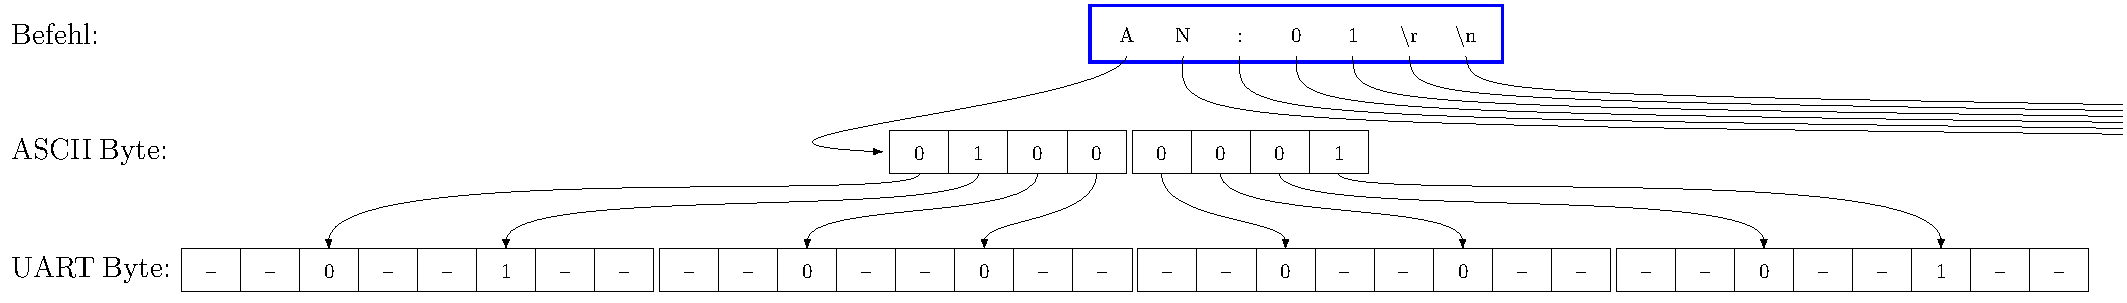
\includegraphics[scale=0.4]{images/UART-Bytes}
    \caption{Umrechnung }
    \label{fig:uart}
  \end{center}
\end{figure}

\subsubsection{libserial}
Das selbst entwickelte C++ Programm nutzt "`liberial"'\footnote{\url{https://github.com/crayzeewulf/libserial}} um sicher und zuverlässig über das Gerätelaufwerk mit dem Arduino (und letztlich dem Kaffeevollautomaten) zu kommunizieren.
Diese Bibliothek bietet eine objektorientierte Schnittstelle für alle \ac{POSIX} Systeme und ist unter Linux über die Paketverwaltung installierbar.
Hiermit konnten die Probleme, bei dem Versuch die Grätedatei direkt anzusprechen (Probleme in Abshnitt \ref{subsec:kommunikationGeraetedateiLibserialLibrary}), gelöst werden.

\subsection{Speicher- und Austauschformat}
Sowohl bei der Untersuchung des Speichers, als auch am Ende für das aufbereitete Ergebnis, werden Informationen gesammelt, verglichen und öffentlich zugäglich gemacht.
Als beliebtes und flexiebles Speichformat wird \ac{JSON} verwendet.
Es bietet viele Datenformate und ist unbegrenzt verschaltelbar.
In dieser Arbeit werden hauptsächlich Zeichenketten, Zahlen und unter Objekte / Arrays verwendet.

Darüber hinaus kann es leicht vom C++ Programm, der Webseite, oder auch für viele weitere Projekte genutzt werden.

\subsubsection{libjsoncpp}
Die "`libjsoncpp"'\footnote{\url{https://en.wikibooks.org/wiki/JsonCpp}} bietet dem C++ Programm eine Lese- und Syntaxanalyse-Funktion zum Aufnehmen eines \ac{JSON} Ausdrucks, sowie eine Möglichkeit ein \ac{JSON} Objekt kompakt zusammengefasst oder leserfreundlich aufgefächert in einen Ausgabestrom zu schreiben.
Als Ausgabestrom sind reine \ac{JSON} Dateien nach einer Speicherauszugs Aufnahme oder die Standardausgabe im Gebrauch als API vorstellbar.


\subsection{Webseite}
Eine kleine Webseite soll am Ende die ausgelesenen Werte visuell anschaulich präsentieren.
Die JavaScript-Bibliothek jQuery und das Framework Bootstrap helfen dabei dies zügig und ansprechend umzusetzen.

\subsubsection{Bootstrap}
Bootstrap\footnote{\url{https://getbootstrap.com/}} ist ein von den Twitter Entwicklern begonnenes Projekt um ursprünglich intern die Verwaltungswerkzeuge zu vereinheitlichen.
Daraus ist aber ein ganzes System an Design Elementen geworden, welches heute sehr populär ist.
\ac{HTML}, \ac{CSS} und \ac{JS} werden zusammen eingesetzt und bieten Entwicklern eine Gitteranordnung für eine Mobile- und die Desktop-Ansicht, Inhaltselemente wie Tabellen und Abbildungen oder auch einzelne Komponenten wie Steckkarten, Prozentanzeigen und Knöpfe.

\subsubsection{jQuery}
jQuery\footnote{\url{https://jquery.com/}} ist eine freie \acl{JS}-Bibliothek, die in der "`slim"'-Variante bereits über Bootstrap eingebunden ist.
Um später wirklich mit dem Kaffeevollautomaten interagieren zu können, wird unter anderem \acs{AJAX} aus dem vollständigen jQuery Paket benötigt (auch wenn daraus später ein synchrones JavaScript mit \acs{JSON} wird).

Über das \acs{CDN} eingebundene Packet stehen ab jetzt einfache \aclp{API} zum modifizieren der \acs{HTML} Elemente, ein erweitertes Event-System, sowie \acs{AJAX}-Funktionalitäten bereit.

\subsubsection{Intro.js}
Zu guter letzt folgt mit Into.js\footnote{\url{https://introjs.com/}} noch eine Schritt-für-Schritt-Anleitung, die dem Seitenbenutzer eine kurze Einführung in den Aufbau und die Bedienung der Webseite geben soll.
